\documentclass{article}
\usepackage{amsmath}
\usepackage{amssymb}
\usepackage{amsthm}
\usepackage{accents}
\usepackage[utf8]{inputenc}
\usepackage{enumitem}
\setlength{\parskip}{1em}
\usepackage{titlesec}
\usepackage{tikz}
\usepackage{physics}

\newcommand{\coord}{co{\"o}rdinate }
\newcommand{\coords}{co{\"o}rdinates }
\newcommand{\bhat}[1]{\boldsymbol{\hat{#1}}}

\newcommand{\ihat}{\ {\hat{\textbf{\i}}}}
\newcommand{\jhat}{\ {\hat{\textbf{\j}}}}
\newcommand{\khat}{\ {\hat{\mathbf{k}}}}
\newcommand{\rhat}{\ {\hat{\mathbf{r}}}}
\newcommand{\that}{\ \boldsymbol{\hat{\theta}}}
\newcommand{\phat}{\ \boldsymbol{\hat{\phi}}}
\newcommand{\rohat}{\ \boldsymbol{\hat{\rho}}}
\newcommand{\zhat}{\ {\hat{\textbf{z}}}}

\renewcommand{\d}{\text{d}}
\renewcommand{\vec}[1]{\accentset{\rightharpoonup}{#1}}

\newcommand{\del}{\vec{\nabla}}
\newcommand{\dvecdot}[2]{\vec{#1}\cdot\d \vec{#2}}
\newcommand{\vecdot}[2]{\vec{#1}\cdot\vec{#2}}

\renewcommand{\curl}[3]{\begin{vmatrix}
    \vspace{0.1cm}
    \ihat & \jhat & \khat\\
    \vspace{0.1cm}
    \pdv{}{x} & \pdv{}{y} & \pdv{}{z}\\
    {#1} & {#2} & {#3}\\
\end{vmatrix}}


\title{Vector Calculus Coursework 2}

\begin{document}

\maketitle

\section*{Question 1}
\subsection*{Part a}

If the closed path (C) does not contain a singularity then the line integral around a closed path for a conservative 
field $\left(\vec{A}\right)$ is zero.
$$\oint_C \dvecdot{A}{l} = 0$$

\subsection*{Part b}
\begin{align*}
    \del F &= \pdv{F}{x}\ihat + \pdv{F}{y}\jhat + \pdv{F}{z}\khat\\
    \del \cross \left(\del F\right) &= \curl{\pdv{F}{x}}{\pdv{F}{y}}{\pdv{F}{z}}\\
    = \ihat\left(\pdv{F}{y}{z} - \pdv{F}{z}{y}\right) + 
    &\jhat\left(\pdv{F}{z}{x} - \pdv{F}{x}{z}\right) +
    \khat\left(\pdv{F}{x}{y} - \pdv{F}{y}{x}\right)\\
    \text{For any function}\quad\quad &\pdv{F}{x}{y} = \pdv{F}{y}{x}\\
    &\pdv{F}{x}{y} - \pdv{F}{y}{x} = 0\\
    &\therefore \del \cross \left(\del F\right) = \ihat(0) + \jhat(0) + \khat(0) = 0
\end{align*}

\subsection*{Part c}
The line integral of $\del F$ around a closed path (C) is zero, this is the same as our conservative field, $\vec{A}$.
$$\oint_C \del F \cdot \text{d}\vec{l}  = \oint_C \dvecdot{A}{l}$$
Therefore we can write our conservative field as a the gradient of a scalar field $\del F = \vec{A}$. We previously
showed that for any $\del F$ the curl is zero therefore
$$\del \cross \vec{A} = \del \cross \left(\del F\right) = 0$$
Therefore a conservative field must always have zero curl. 

\subsection*{Question 2}
\subsection*{Part a}
\begin{center}
    \begin{tikzpicture}[x=2cm, y=2cm]
        \draw[->] (0,0) -- (0,2.5) node[anchor=mid east]{$y$};
        \draw[->] (0,0) -- (2.5,0) node[anchor=north]{$x$};
        \draw[thick] (0,0) -- (1,2) node[anchor=west,midway]{$1$} node[anchor=west]{$(1,2)$};
        \draw[thick,->] (0,0) -- (0.5,1);
        \draw[thick] (1,2) -- (0,2) node[anchor=north,midway]{$2$} node[anchor=east]{$(0,2)$};
        \draw[thick,->] (1,2) -- (0.5,2);
        \draw[thick] (0,2) -- (0,0) node[anchor=east,midway]{$3$} node[anchor=east]{$(0,0)$};
        \draw[thick,->] (0,2) -- (0,1);
    \end{tikzpicture}
\end{center}

\begin{align*}
    \vec{A} &= xy\ihat + \jhat\\
    \d \vec{l} &= \d x\ihat + \d y\jhat\\
    \dvecdot{A}{l} &= xydx + dy\\ 
\end{align*}

\subsubsection*{Side 1}
We can represent this side as a path of equation $y = 2x$, where the bounds for such a path are 
$x: 0 \rightarrow 1,\ y: 0 \rightarrow 2$

\begin{align*}
    \int \dvecdot{A}{l} &= \int_0^1 xy \d x + \int_0^2\d y\\
    y = 2x &\therefore xy = 2x^2\\
    \int_0^1 2x^2 \d x + \int_0^2\d y &= \left[\frac{2}{3}x^3\right]_0^1 + 2\\
    &= \frac{2}{3} + 2 = \frac{8}{3}\\
\end{align*}

\subsubsection*{Side 2}
For this side $y = 2$ for the entire length, so we can make that substitution.
\begin{align*}
    \int \dvecdot{A}{l} &= \int_1^0 2x \d x + \int_2^2\d y\\
    &= \left[x^2\right]_1^0 = -1
\end{align*}

\subsubsection*{Side 3}
$x = 0$ for this side, so this simplifies the integral a lot

\begin{align*}
    \int \dvecdot{A}{l} = \int_2^0\d y = -2
\end{align*}

Summing all of the sides will gives us the final answer for our path integral
$$\oint \dvecdot{A}{l} = \frac{8}{3} - 1 - 2 = \frac{-1}{3}$$

\subsection*{Part b}

\begin{align*}
    \del \cross \vec{A} &= \curl{xy}{1}{0}\\
    &= \khat(\pdv{}{x}1 - \pdv{}{y}xy) \\
    &= -\khat x
\end{align*}

\subsection*{Part c}
$\vec{A}$ is non-conservative, neither its cross product nor its closed path integral are zero.

\section*{Question 3}
\subsection*{Part a}
The magnetic field is symmetrical up and down in the $z$ direction, so $z$ does not matter.
It is directed in \emph{circles} (meaning it is pointed in the $\phat$ direction) around the wire, 
implying that for a certain magnitude ($B$) it is at a fixed radius ($\rho$). Given all of this we can state
that $\vec{B}(\rho) \phat$, $\vec{B}$ is a function of $\rho$ pointed in the $\phat$ direction. 

\begin{align*}
    \d \vec{l} &= \d\rho\rohat + \rho \d \phi\phat + \d z\zhat\\
    \oint_C \dvecdot{B}{l} &= \int_0^{2\pi} B \cdot \rho\,\d\phi\\
    &= 2\pi\rho B = \mu_0 I\\
    B &= \frac{\mu_0 I}{2\pi\rho}\\
    \text{We stated previously that}\quad \vec{B} &= B\phat \\
    \vec{B} &= \frac{\mu_0 I}{2\pi\rho} \phat
\end{align*}

\subsection*{Part b}
\begin{align*}
    \rho &= \sqrt{x^2+y^2}\\
    \phat &= -\sin \phi \ihat + \cos\phi \jhat\\
    \vec{B} &= \frac{\mu_0 I}{2\pi\sqrt{x^2+y^2}} \left(-\sin \phi \ihat + \cos\phi \jhat\right)\\
    \sin\psi &= \frac{y}{\rho}\\
    \cos\psi &= \frac{x}{\rho}\\
    \vec{B} &= \frac{(-y + x)\mu_0 I}{2\pi (x^2+y^2)}\\
    \dvecdot{B}{l} &= \frac{-y \mu_0 I}{2\pi (x^2+y^2)} \d x + \frac{x \mu_0 I}{2\pi (x^2+y^2)} \d y\\
    \text{let}\quad k &= \frac{\mu_0 I}{2\pi}\\
    &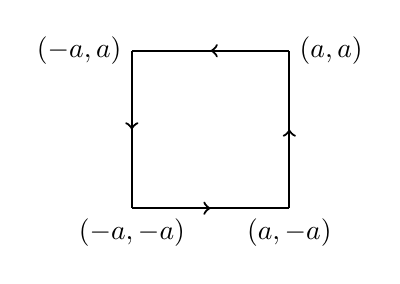
\begin{tikzpicture}[x=2cm, y=2cm]
        \draw[thick] (0,0) -- (1,0) node[anchor=north,midway]{$$} node[anchor=north]{$(a, -a)$};
        \draw[thick,->] (0,0) -- (0.5,0);
        \draw[thick] (1,0) -- (1,1) node[anchor=west,midway]{$$} node[anchor=west]{$(a, a)$};
        \draw[thick,->] (1,0) -- (1,0.5);
        \draw[thick] (1,1) -- (0,1) node[anchor=south,midway]{$$} node[anchor=east]{$(-a, a)$};
        \draw[thick,->] (1,1) -- (0.5,1);
        \draw[thick] (0,1) -- (0,0) node[anchor=east,midway]{$$} node[anchor=north]{$(-a, -a)$};
        \draw[thick,->] (0,1) -- (0,0.5);
    \end{tikzpicture}\\
    &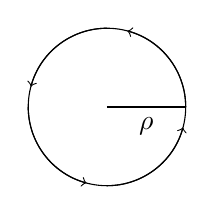
\begin{tikzpicture}
        \draw(0,0) circle (1cm);
        \draw[thick] (0,0) -- (1,0) node[anchor=north,midway]{$\rho$};
        \draw[->] (1, 0) arc (0:75:1cm);
        \draw[->] (-1, 0) arc (180:180+75:1cm);
        \draw[->] (0, 1) arc (90:90+75:1cm);
        \draw[->] (0, -1) arc (270:270+75:1cm);
    \end{tikzpicture}\\
\end{align*}
Let's consider a side going from $(a,-a)$ to $(a,a)$, this side has a constant $x$ value, which means that 
the integral with respect to $x$ is 0.
\begin{align*}
    \int \dvecdot{B}{l} &= k \int_{-a}^a \frac{x}{x^2+y^2}\d y\\
    x &= a\\
    \int \dvecdot{B}{l} &= k \int_{-a}^a \frac{a}{a^2+y^2}\d y\\
    \text{let}\quad y &= au\\
    \int \dvecdot{B}{l} &= k \int_{-a}^a \frac{a}{a^2(1+u^2)}\d y\\
    \dv{y}{u} &= a\\
    \int \dvecdot{B}{l} &= k \int_{-a}^a \frac{a^2}{a^2(1+u^2)} \d u\\
    &= k \int_{-a}^a \frac{1}{(1+u^2)} \d u\\
    \text{using integral identity }\quad &= k \left[\arctan\left(\frac{y}{a}\right)\right]_{-a}^{a} \\
    &= k (\arctan(1) - \arctan(-1)) = k\frac{1}{2}\pi
\end{align*}
Now if we consider the side opposite to this one, going from $(-a, a)$ to $(-a, -a)$ we can see that $x$ is still 
a constant but this time it's equal to $-a$, this is convinient since the bounds for this integral are reversed.
It is known for any integral that 
$$\int_a^b \d x =  - \int_b^a \d x$$
Thus we can say that these sides have an equal line integral, $k\frac{1}{2}\pi$.
\newline

Now let's consider the top side, from $(a, a)$ to $(-a, a)$, for this side $y = a$, and so any integral with 
respect to $y$ is just 0. 
\begin{align*}
    \int \dvecdot{B}{l} &= k \int_{a}^{-a} \frac{-y}{x^2+y^2}\d x\\
    \text{let}\quad x &= au\\
    \int \dvecdot{B}{l} &= k \int_{a}^{-a} \frac{-1}{(1+u^2)}\d u\\
    &= k \int_{-a}^{a} \frac{1}{(1+u^2)}\d u\\
    &= k \left[\arctan\left(\frac{x}{a}\right)\right]_{-a}^{a} \\
    &= k (\arctan(1) - \arctan(-1)) = k\frac{1}{2}\pi\\
\end{align*}

Using the same logic, the opposite side is the same except the bounds are reversed ($-a \rightarrow a$),
and $y = -a$, these both "cancel" each other to give the same answer to the integral as previously. 
Summing all of these sides together gives us an answer of 
\begin{align*}
    \oint_C \dvecdot{B}{l} = k2\pi = \frac{\mu_0 I 2\pi}{2\pi} = \mu_0 I
\end{align*}
Hence, this obeys Ampère's Law. 

\subsection*{Part c}
A field is conservative if $\del \cross \vec{B} = 0$.

\begin{align*}
    \del \cross \vec{B} &= \frac{1}{\rho}
    {\begin{vmatrix}
        \vspace{0.1cm}
        \rohat & \rho {\mkern-6mu} \phat & \zhat\\
        \vspace{0.1cm}
        \pdv{}{\rho} & \pdv{}{\phi} & \pdv{}{z}\\
        {0} & \frac{\mu_0 I}{2\pi} & 0\\
    \end{vmatrix}} = 0\\
\end{align*}
$\frac{\mu_0 I}{2\pi}$ is a constant (for a certain $I$) and so any derivative of it will always be zero, 
thus the field is conservative outside of the wire. 

\end{document}